\documentclass[12pt, a4paper, twoside]{article}
\usepackage{../labreport}
\usepackage{pdfpages}

\setlabreportopts[authors={Nandor Kovacs \& Céline Schuster},
    title={Mathematisches Pendel},
    subtitle={Untersuchung der Eigenschaften eines Mathematischen Pendels},
    date={\today},
    labdate={10. März 2022}
]

\begin{document}
\maketitlepage
\includepdf[pages=2-3]{aufgabenstellung.pdf}

\section{Einleitung}
\section{Theorie}
\section{Demo 1}
\section{Demo 2}
\section{Versuch 1}
\subsection{Experimentbeschreibung}
In einer Entfernung von 20cm zum Zählrohr wird eine radioaktive Quelle platziert.
Die Schutzkappe wird von der Quelle entfernt.
Nun wird dreimal die Zeit gemessen, in der 1000 Erreignisse geschehen.
Das gleiche Experiment wird auch in einer Entfernung von 10cm ausgeführt.
\subsection{Aufgabe 1}

\subsection{Aufgabe 2}

\subsection{Aufgabe 3}

\section{Versuch 2}
Es wird 20mal mit 24 Würfeln gewürfelt.
Nach jedem Wurf wird gezählt, wie viele Würfel die Augenzahl Sechs aufweisen.

\datatable{c}{\csvcoli}{Würfelwürfe}{Anzahl 6er $W$}{wurfel.csv}{wurfel};
\subsection{Aufgabe 1}
Der Median $m$ unserer Würfelwürfe:
\begin{align*}
  m & = \frac{\sum_{i=1}^{n} W_{i}}{n} \\
  m & = \frac{79}{20}                  \\
  m & =3.95                            \\
\end{align*}
Die Chance das ein Würfel die Augenzahl 6 hat, ist $\frac{1}{6}$.
Der Erwartungswert $E$ ist gleich der Anzahl Würfel, mal die Wahrscheinlichkeit für eine 6:
\begin{align*}
  E & = 24 \cdot \frac{1}{6} \\
  E & = \frac{24}{6}         \\
  E & = 4;
\end{align*}
Der Wert $m$ ist nahezu gleich zu $E$.

Der Wert maximaler Häufigkeit ist 9.


\section{Versuch 3}

\section{Fazit}
\section{Reflektion}



\end{document}
